\documentclass[a4paper,12pt, oneside]{article}

\title{\textbf{L'impatto del Codec AV1 sull'industria della visualizzazione online} \\ \large A.A 2023/2024 \\ Elaborato di Crittografia}
\author{Gabos Norbert \\ 0000970451 \\ tiberiunorbert.gabos@studio.unibo.it }
\date{}

\usepackage[T1]{fontenc}
\usepackage[utf8]{inputenc}
\usepackage[italian]{babel}
\pagestyle{plain}
\usepackage{graphicx}
\usepackage[table,xcdraw]{xcolor}
\usepackage{tabularx}
\usepackage{ragged2e}               % migliora la formattazione del testo all'interno delle celle
\renewcommand{\arraystretch}{1.5}   % aggiunge margine alle celle
\graphicspath{{images/}}

\definecolor{darkBlue}{RGB}{21, 69, 179}
\definecolor{lightPink}{RGB}{242, 10, 172}

\begin{document}

\maketitle

\newpage
\tableofcontents{}
\newpage

\section{Introduzione}
Con l'avvento dei computer e la crescente digitalizzazione dei media, è emersa la necessità di
trovare soluzioni efficaci per rappresentare e archiviare i video all'interno dei sistemi
informatici. Questo processo ha comportato la trasformazione dei tradizionali filmati in una
forma compatibile con il mondo digitale, dove ogni istante del video è rappresentato da una
sequenza di immagini statiche, comunemente note come frame. Ogni frame, a sua volta, è
composto da una matrice di pixel, gli elementi fondamentali che compongono l'immagine, ognuno
dei quali è definito da una terna di colori \textbf{RGB} (Red, Green, Blue) e da una profondità
di colore che varia generalmente tra 0 e 255.

Questo approccio ha permesso di preservare la qualità visiva dei contenuti video e di renderli
compatibili con le capacità di elaborazione dei computer. Tuttavia, la mera rappresentazione
dei video in questo modo ha portato ad un'elevata quantità di dati da gestire ed archiviare
comportando sfide significative in termini di spazio di archiviazione e larghezza di banda.
Per esempio un banale video da 10 minuti in 1080p a 30 fotogrammi al secondo pesa
all'incirca 111 GB.
\noindent
\\\\Peso\_video = Risoluzione × Fotogrammi\_al\_secondo × Durata × Profondità\_colore\\

Questo rappresentava un enorme problema in quanto i dispositivi dell'epoca riuscivano ad
immagazzinare solo una manciata di MB. Problema che persiste tutt'oggi in quanto le esigenze
di qualità video sono aumentate di molto, nonché il numero di dispositivi che creano contenuti
multimediali regolarmente, quindi molti più video.
Per affrontare queste sfide e ottimizzare l'archiviazione e la trasmissione dei video
digitali, sono stati sviluppati una serie di algoritmi e standard di compressione video.
Esistono due approcci principali alla compressione video: la compressione \textbf{lossless} e
la compressione \textbf{lossy}. La compressione lossless, ad esempio con algoritmi come
\textbf{Huffyuv} e \textbf{Lagarith}, mira a ridurre le dimensioni del file senza perdita di
qualità, mantenendo ogni singolo dato originale. D'altro canto, la compressione lossy
sacrifica una certa quantità di qualità visiva per raggiungere una maggiore compressione dei
dati, consentendo una gestione più efficiente delle risorse di archiviazione e una
trasmissione più rapida attraverso le reti digitali.

In questa relazione, esploreremo l'evoluzione della compressione video lossy, partendo dal
contesto della sua necessità fino alla discussione di algoritmi più recenti e avanzati come il
Codec AV1. Analizzeremo come questi algoritmi hanno rivoluzionato il modo in cui i video
vengono elaborati, archiviati e trasmessi sui mezzi digitali, con un focus particolare sugli
impatti e le potenzialità di tali innovazioni nell'industria multimediale moderna.

\section{I primi passi}
\subsection{H.261}
Nel 1988 nasce il codec H261 che è stato il primo algoritmo di compressione video ad utilizzare
in modo efficiente degli algoritmo di \textbf{intraframe} e \textbf{interframe}, che sono
spiegati nel paragrafo successivo, ed è responsabile dell'introduzione della codifica video
ibrida basata su blocchi, che è ancora utilizzata oggi in molti standard video.
\noindent
\\\\\textbf{Intraframe}: L'intraframe compression, o compressione intra-frame, si riferisce alla
compressione dei dati all'interno di un singolo fotogramma. Questo metodo sfrutta le ridondanze
spaziali all'interno di un singolo frame.
\\\\\textbf{Interframe}: L'interframe compression, o compressione inter-frame, lavora sulla
ridondanza temporale tra i frame adiacenti. Invece di codificare ogni frame singolarmente,
vengono identificate e codificate solo le differenze tra i frame successivi o precedenti.
Questo consente di ridurre ulteriormente le dimensioni del file video, poiché molte
informazioni rimangono costanti tra i fotogrammi vicini.
\noindent
\\\\Prima di proseguire, visto che non parliamo più dei video come una matrice di pixel, ma più di
un flusso di dati, bisogna introdurre il concetto di bitrate.
Il \textbf{bitrate} è una misura della velocità di trasmissione dei dati in un file multimediale,
come un video o un brano audio. Rappresenta quanti dati vengono trasmessi o elaborati in un
determinato intervallo di tempo espresso in \textbf{bit/s}. In generale, a parità di tecnologie
utilizzate per la compressione, più il bitrate di un contenuto è elevato e più la sua qualità
sarà maggiore al costo di un peso più elevato. Vedi Figura~\ref{fig:confronto_bitrate}.

\begin{figure}[ht]
    \centering
    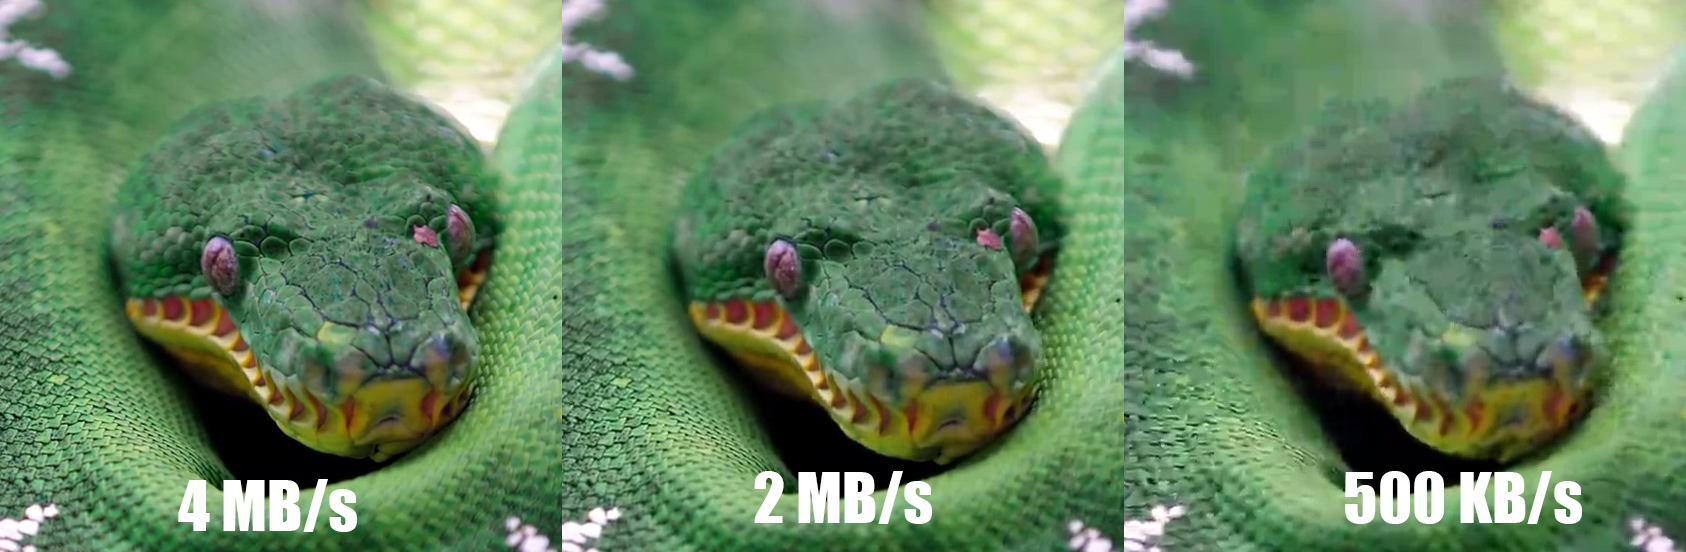
\includegraphics[width=1\textwidth]{images/confronto-bitrate.png}
    \caption{L'immagine mette a confronto 3 frame presi allo stesso istante da un video compresso con 3 valori di bitrate differenti.}
    \label{fig:confronto_bitrate}
\end{figure}

TODO: Magari si potrebbero spiegare meglio queste due tecniche più avanti nell'articolo, quindi sarebbe meglio scrivere in questo
punto che questi due algoritmi verranno spiegati meglio nei paragrafi successivi

\section{Tecnologie attuali}
\subsection{H.264 e H.265}
TODO: L'h264 essendo una tecnica che racchiude molti algoritmi complessi per la compressione video, necessita di accelleratori hardware per poter decodificare i fotogrammi in tempo reale.

\subsection{VP9}    % forse non serve descriverlo
\subsection{AV1}
\subsection{Comparazione delle prestazioni}

\section{Vantaggi per le aziende}

\section{Sfide e considerazioni}
Non dimenticare di discutere anche delle sfide e delle considerazioni pratiche legate all'adozione di nuovi codec, come il supporto hardware/software, la compatibilità con dispositivi esistenti e la gestione dei diritti d'autore.

\section{Conclusioni}

\section{Bibliografia}
\\-parla dei tecnicismi del h.261 https://users.ece.utexas.edu/~ryerraballi/MSB/pdfs/M4L2.pdf
\\-bitrate https://it.wikipedia.org/wiki/Velocit%C3%A0_di_trasmissione
\\-sito ufficiale di h.265 https://hevc.hhi.fraunhofer.de/
\\-repository di h.265 https://vcgit.hhi.fraunhofer.de/jvet/HM
\\-sito che parla della storia degli encorder https://api.video/blog/video-trends/the-history-of-video-compression-starts-in-1929/
\\-utile! parla dei tecnicismi del h.264 nella sezione di Implementing h.264 https://www.embedded.com/implementing-h-264-video-compression-\\algorithms-on-a-software-configurable-processor/
\\-utile! parla dei tecnicismi del h.265 nella sezione di Coding tools https://en.wikipedia.org/wiki/High_Efficiency_Video_Coding

\end{document}
